\documentclass[12pt]{article}
\usepackage{amsmath}
\usepackage{amssymb}
\usepackage{amsthm}
\usepackage[left=2cm, right=2cm, top=2cm]{geometry}
\usepackage{enumitem}
\usepackage{graphicx}
\usepackage{color}   %May be necessary if you want to color links
\usepackage{hyperref}
\hypersetup{
    colorlinks=true, %set true if you want colored links
    linktoc=all,     %set to all if you want both sections and subsections linked
    linkcolor=blue,  %choose some color if you want links to stand out
}
\usepackage{bbm}
\usepackage{soul}
\usepackage{tcolorbox}
\usepackage{tikz}
\tcbuselibrary{theorems}
\tcbuselibrary{breakable}

\newtcbtheorem[number within=section]{mythm}{Theorem}%
{colback=green!5,colframe=green!35!black,fonttitle=\bfseries,unbreakable}{th}
\newtcbtheorem[use counter from=mythm]{mydef}{Definition}%
{colback=blue!5,colframe=blue!35!black,fonttitle=\bfseries,unbreakable}{de}
\newtcbtheorem[use counter from=mythm]{myrem}{Remark}%
{colback=white!5,colframe=white!35!black,fonttitle=\bfseries,unbreakable}{re}
\newtcbtheorem[use counter from=mythm]{myex}{Example}%
{colback=orange!5,colframe=orange!35!black,fonttitle=\bfseries,unbreakable}{ex}
\newtcbtheorem[use counter from=mythm]{myprop}{Proposition}%
{colback=green!5,colframe=green!35!black,fonttitle=\bfseries,unbreakable}{pr}
\newtcbtheorem[use counter from=mythm]{mylem}{Lemma}%
{colback=green!5,colframe=green!35!black,fonttitle=\bfseries,unbreakable}{le}
\newtcbtheorem[use counter from=mythm]{mycor}{Corollary}%
{colback=green!5,colframe=green!35!black,fonttitle=\bfseries,unbreakable}{co}

\newcommand{\R}{\mathbb{R}}
\newcommand{\N}{\mathbb{N}}
\newcommand{\Z}{\mathbb{Z}}
\newcommand{\Q}{\mathbb{Q}}
\renewcommand{\C}{\mathbb{C}}
\newcommand{\inv}{^{-1}}

\setcounter{tocdepth}{3}
\setlength\parindent{0pt}
\hyphenpenalty 10000

\title{PMATH 336 Course Notes - Spring 2019}
\author{Max Zhu}

\begin{document}
	\maketitle
	\tableofcontents\newpage
	
	\section{Groups}
	\subsection{Definition and simple examples}
	Groups are used for describing symmetries of objects, and for finding solutions to equations. Before formally defining what a group is, we will start with some examples and note their properties.
	\begin{myex}{Integers with addition}{}
		$(\Z, +)$, the integers with usual addition, is a group. We notice the following properties.
		\begin{itemize}
			\item For all $a, b\in\Z$ we have $a+b\in\Z$. \textbf{(closure)}
			\item There is an identity $0\in\Z$ such that for all $a\in\Z$, we have $a+0=0+a=a$. \textbf{(identity)}
			\item Every integer $a\in\Z$ has an inverse $a\inv\in\Z$ such that $a+a\inv=a\inv+a=0$. Here, $a\inv=-a$. \textbf{(inverses)}
			\item Let $a, b, c\in\Z$. Then, $(a+b)+c=a+(b+c)$. \textbf{(associativity)}
		\end{itemize}
	\end{myex}
	
	\begin{myex}{Rationals with addition}{}
		$(\Q, +)$, rational numbers with usual addition, is a group. Similarly to the integers,
		\begin{itemize}
			\item For all $a, b\in\Q$ we have $a+b\in\Q$. \textbf{(closure)}
			\item There is an identity $0\in\Q$ such that for all $a\in\Q$, we have $a+0=0+a=a$. \textbf{(identity)}
			\item Every integer $a\in\Q$ has an inverse $a\inv\in\Q$ such that $a+a\inv=a\inv+a=0$. Here, $b=-a$. \textbf{(inverses)}
			\item Let $a, b, c\in\Q$. Then, $(a+b)+c=a+(b+c)$. \textbf{(associativity)}
		\end{itemize}
	\end{myex}
	\begin{myex}{Real and complex numbers with addition}{}
		$(\R, +)$ and $(\C, +)$ are also groups, and these properties can be verified.
	\end{myex}
	
	\begin{myex}{}{}
		$(\{1, 1, i, -i\}, \cdot)$ is a group. We can create a table to show the result of the operation on any two elements of the set:
		\begin{align*}
			\begin{array}{c | cccc}
			\cdot & 1  & -1 & i  & -i \\
			\hline
			1     & 1  & -1 & i  & -i \\
			-1    & -1 & 1  & -i & i  \\
			i     & i  & -i & -1 & 1  \\
			-i    & -i & i  & 1  & -1
			\end{array}
		\end{align*}
		This kind of table is called a \underline{Cayley table}.
		\begin{itemize}
			\item Note that each row and column contains each element exactly once.
			\item From the Cayley table, the set is closed under $\cdot$.
			\item The identity is 1.
			\item Each element has an inverse in the set:\begin{align*}
				(1)\inv&=1\\
				(-1)\inv&=-1\\
				(i)\inv&=-i\\
				(-i)\inv&=i
			\end{align*}
		\end{itemize}
	\end{myex}
	
	\begin{mydef}{Group}{}
		Let $G$ be a set, and $\star:G\times G\to G$ be a binary operation on $G$. We say $(G, \star)$ is a \underline{group} if it satisfies the following conditions:
		\begin{enumerate}[label=(\roman*)]
			\item \underline{Associativity:} Let $a, b\in G$. Then, $(a\star b)\star c)=a\star(b\star c)$.
			\item \underline{Identity:} There exists $e\in G$ such that for all $a\in G$, we have $a\star e=e\star a=a$.
			\item \underline{Inverses:} For all $a\in G$, there exists $a\in\in G$ such that $a\star a\inv=a\inv\star a=e$.
		\end{enumerate}
	\end{mydef}
	
	\begin{myrem}{}{}
		\begin{itemize}
			\item When proving a set $G$ with an operation $\star$ is a group, we must also show $G$ is closed under $\star$.
			\item We often refer to a group $(G, \star)$ as simply $G$.
			\item We often write $ab$ instead of $a\star b$ for some operation $\star$.
			\item We usually denote the identity element of a group with $e$.
		\end{itemize}			
	\end{myrem}
	
	\begin{myprop}{Nonzero rationals with multiplication is a group}{}
		$(\Q\backslash\{0\}, \cdot)$, nonzero rationals with usual multiplication, is a group. 
		\begin{proof}
			We use the notation $\Q^*:=\Q\backslash\{0\}$.
			
			Let $a, b, c, d, e, f\in\Z$ so $\frac{a}{b}, \frac{c}{d}, \frac{e}{f}\in\Q^*$. Then,
			\begin{enumerate}[label=(\roman*)]
				\item $\frac{a}{b}\cdot\frac{c}{d}=\frac{ac}{bd}\in\Q^*$ \textbf{(closure)}
				\item $\frac{a}{b}\cdot(\frac{c}{d}\cdot\frac{e}{f})=(\frac{a}{b}\cdot\frac{c}{d})\cdot\frac{e}{f}$ \textbf{(associativity)}
				\item $\frac{1}{1}\cdot\frac{a}{b}=\frac{a}{b}\cdot\frac{1}{1}=\frac{a}{b}$ \textbf{(identity)}
				\item $\frac{a}{b}\cdot\frac{b}{a}=\frac{b}{a}\cdot\frac{a}{b}=\frac{1}{1}$, and $\frac{b}{a}\in\Q^*$ \textbf{(inverses)}
			\end{enumerate}
			So, $(\Q^*, \cdot)$ has all required properties of a group.
		\end{proof}
	\end{myprop}
	
	\begin{myex}{Integers modulo n with addition}{}
		$(\Z_n, +)$, integers modulo n with addition is a group.
		
		Here, $\Z_n=\{[0], \dots, [n-1]\}$ where $[a]=\{b\in\Z:b\text{ has remainder $a$ when dividing by n}\}$, and $[a]+[b]=[a+b]$. To save space, we may write $a$ instead of $[a]$. Let us use $\Z_5$ as an example.\\
		
		$\Z_5=\{0, 1, 2, 3, 4\}$. Here is the Cayley table for $\Z_5$:
		\begin{align*}
			\begin{array}{c | ccccc}
			+ & 0 & 1 & 2 & 3 & 4 \\
			\hline
			0 & 0 & 1 & 2 & 3 & 4 \\
			1 & 1 & 2 & 3 & 4 & 0 \\
			2 & 2 & 3 & 4 & 0 & 1 \\
			3 & 3 & 4 & 0 & 1 & 2 \\
			4 & 4 & 0 & 1 & 2 & 3
			\end{array}
		\end{align*}
		We can quickly verify the 4 properties. Let $[a], [b], [c]\in\Z_5$. Then,
		\begin{enumerate}[label=(\roman*)]
			\item Closure: obvious from the Cayley table.
			\item Associativity: $[a]+([b]+[c])=[a]+[b+c]=[a+b+c]=[a+b]+c=([a]+[b])+c$
			\item Identity: $[0]+[a]=[0+a]=[a]=[a+0]=[a]+[0]$
			\item Inverses: $[a]\inv=[-a]=[n-a]$
		\end{enumerate}
	\end{myex}
	
	\begin{myex}{``Integers modulo n" with multiplication}{}
		$(\Z_n^*, \cdot)$, where $\Z_n^*:=\{[a]\in\Z_n:\gcd(a, n)=1\}$ and $[a]\cdot[b]=[ab]$, is a group. Let us use $\Z_6^*$ as an example.\\
		
		$\Z_6^*=\{1, 5\}$. Note, $4\notin\Z_6^*$ since $2|4$ and $2|6$, so $\gcd(4, 6)=2\neq1$. Here is the Cayley table for $\Z_6^*$:
		\begin{align*}
			\begin{array}{c | cc}
			\cdot & 1 & 5 \\
			\hline
			1     & 1 & 5 \\
			5     & 5 & 1
			\end{array}
		\end{align*}
		Here, the identity is $1$ and the inverses are $(5)\inv=5$ and $(1)\inv=1$.
	\end{myex}
	
	\begin{myex}{General linear group in $\R$}{}
		We define the group $GL_n(\R)$ to be the set $\{A\in M_n(\R):\det(A)\neq0\}$ with usual matrix multiplication. We can easily verify the properties. Let $A, B\in GL_n(\R)$. Then,
		\begin{enumerate}[label=(\roman*)]
			\item Closure: $\det(AB)=\det(A)\det(B)\neq0$ so $AB\in GL_n(\R)$.
			\item Associativity: matrix multiplication is known to be associative.
			\item Identity: $\det(I)=1\neq0$ where $I=\begin{bmatrix}1&~&0\\~&\ddots\\0&~&1\end{bmatrix}$ is the identity matrix.
			\item Inverses: usual matrix inverses, since $\det(A\inv)=\frac{1}{\det(A)}\neq0$ so $A\inv\in GL_n(\R)$.
		\end{enumerate}
	\end{myex}
	
	\begin{mydef}{Abelian groups}{}
		A group $(G, \star)$ is \underline{abelian} if for all $a, b\in G$ we have $a\star b=b\star a$. Otherwise, the group is \underline{non-abelian}.	
	\end{mydef}
	
	\begin{myex}{Some abelian groups}{}
		$(\Z, +), (\Q^*, \cdot), (\Z_n, +), (\Z_n^*)$ are all abelian.
	\end{myex}
	
	\begin{myex}{Dihedral groups}{}
		\underline{Dihedral groups}	$(D_n, \cdot)$ are a family of groups of symmetries of a regular n-gon. The operations can be thought of as operations that change places of the vertices but not the overall shape of the polygon. Let us use $D_4$ as an example.\\
		
		$D_4$ is the group of symmetries of a square. Elements of $D_4$ include:
		\begin{itemize}
			\item $e$, rotation by 0\textdegree.
			\item $R$, rotation by 90\textdegree counter-clockwise.
			\item $R^2$, rotation by 180\textdegree counter-clockwise.
			\item $R^3$, rotation by 270\textdegree counter-clockwise.
		\end{itemize}
		We also have flips:
		\begin{itemize}
			\item $H$, flip through horizontal axis.
			\item $V$, flip through vertical axis.
			\item $D$, flip through top-left bottom-right diagonal axis.
			\item $D'$, flip through top-right bottom-left diagonal axis.
		\end{itemize}
		The elements are functions from a set of vertices to itself which preserves distance and adjacent-ness. The operator is composition of functions. For example, $HR$ is application of $R$ then $H$.
		
		\includegraphics[scale=0.3]{Fig1.png}
		
		From this MS Paint illustration of some operations in $D_4$, it is clear that $D_4$ is non-abelian.
	\end{myex}
	
	\begin{mydef}{Order of a group}{}
		Let $(G, \star)$ be a group. The \underline{order} of $G$ is the number of elements in $G$, which is denoted $|G|$. If $G$ is infinite, we say $|G|=\infty$.	
	\end{mydef}
	
	\begin{myex}{Orders of some groups}{}
		\begin{align*}
			|Z_n|&=n\\
			|Z_n^*|&=\phi(n)\text{ (Euler's totient function)}\\
			|(\Z, +)|&=\infty\\
			|D_n|&=2n
		\end{align*}			
	\end{myex}
	
	\subsection{Properties of groups}
	\begin{myprop}{Uniqueness of identity}{}
		In a group $G$, there is only one identity element.
		\begin{proof}
			Assume there are 2 identities $e, f\in G$. Since $e$ is an identity,
			\begin{align*}
				ef=fe&=f
			\end{align*}
			And since $f$ is an identity,
			\begin{align*}
				fe=ef&=e
			\end{align*}
			Therefore $e=f$.
		\end{proof}			
	\end{myprop}
	
	\begin{myprop}{Cancellation}{}
		If $G$ is a group, for all $a, b, c\in G$ we have:
		\begin{align*}
			ab=ac&\Longrightarrow b=c\text{ [Left cancellation]}\\
			ba=ca&\Longrightarrow b=c\text{ [Right cancellation]}
		\end{align*}
		\begin{proof}
			Let $a, b, c\in G$ such that $ab=ac$. Then,
			\begin{align*}
				ab&=ac\\
				a\inv(ab)&=a\inv(ac)\\
				(a\inv a)b&=(a\inv a)c\text{ [associativity]}\\
				eb&=ec\text{ [inverses]}\\
				b&=c\text{ [identity]}
			\end{align*}
			As required. Right cancellation has similar proof.
		\end{proof}
	\end{myprop}
	
	\begin{myrem}{}{}
		Cancellation should be on the same side. For example in $D_4$, $RH=D'=VR$ but $H\neq V$.	
	\end{myrem}
	
	\begin{myprop}{Uniqueness of inverses}{}
		Let $G$ be a group. If $b, c$ are both inverses of $a$ then $b=c$.
		\begin{proof}
			Suppose $e=ab=ac$. Then,\begin{align*}
				ab&=ac\\
				b(ab)&=b(ac)\\
				(ba)b&=(ba)c\text{ [associativity]}\\
				eb&=ec\text{ [by hypothesis]}\\
				b&=c\text{ [identity]}
			\end{align*}
			as required.
		\end{proof}	
	\end{myprop}
	
	\begin{myprop}{Socks-shoes}{}
		Let $G$ be a group with $a, b\in G$. Then, $(ab)\inv=b\inv a\inv$.
		\begin{proof}
			\begin{align*}
				(ab)(b\inv a\inv)&=a(bb\inv)a\inv\\
				&=a(ea\inv)\\
				&=aa\inv\\
				&=e
			\end{align*}
			so $(ab)\inv=b\inv a\inv$ as required.
		\end{proof}			
	\end{myprop}
	
	\begin{mydef}{Exponentiation}{}
		Let $(G, \star)$ be a group, with $a\in G$, $n\in\Z$. Then,
		\begin{align*}
			a^n:=\begin{cases}
				a\star\dots\star a\text{ (n times)},&n>0\\
				e,&n=0\\
				a\inv\star\dots\star a\inv\text{ (n times)},&n<0
			\end{cases}
		\end{align*}
		
		Note: some exponential properties work with the same base. For example,
		\begin{align*}
			a^na^m&=a^{n+m}\\
			(a\inv)^n&=a^{-n}
		\end{align*}
		However, in general $(ab)^n\neq a^nb^n$ for $a. b\in G$ unless $G$ is abelian.
	\end{mydef}
	
	\begin{mydef}{Order of an element}{}
		Let $G$ be a group with $a\in G$. The \underline{order} of $a$ is the smallest positive integer such that $a^k=e$. We denote this by $|a|=k$. If $a^k\neq e$ for all $k$, we say $|a|=\infty$.
	\end{mydef}
	
	\begin{myex}{Some orders of group elements}{}
		\begin{itemize}
			\item In all groups, $|e|=1$\\
			\item In $D_4$, $|v|=2$\\
			\item In $\Z_{15}^*$, $|z|=4$\\
			\item In $\Z$, all nonzero elements have order $\infty$\\
			\item In $\Q^*$, $|1|=1$ and $|-1|=2$
		\end{itemize}			
	\end{myex}
	
	\begin{mydef}{Direct products}{}
		Let $(G, \star), (H, \cdot)$ be groups. Then, the set $G\times H=\{(g, h):g\in G, h\in H\}$ with operation $(g_1, h_1)\Delta(g_2, h_2):=(g_1\star g_2, h_1\cdot h_2)$ is a group. $(G\times H, \Delta)$ is called the \underline{direct product} of $G$ and $H$.
	\end{mydef}
	
	\section{Subgroups}
	\begin{mydef}{Subgroup}{}
		Let $(G, \star)$ be a group, and $H\subseteq G$. Then $H$ is a \underline{subgroup} of $G$ if $(H, \star)$ is a group.\\
		
		If $H$ is a subgroup of $G$, we say $H\leq G$ and if $H\subsetneq G$, we say $H<G$.\\
		
		If 	$(H, \star)$ is not a group, we say $H\nleq G$.
	\end{mydef}
	
	\begin{myex}{Some easy subgroups}{}
		For all groups $(G, \star)$, we know $\{e\}\leq G$ and $G\leq G$.
	\end{myex}
	
	\begin{myex}{Subgroups of $\Z$}{}
		Define $n\Z=\{nk:k\in\Z\}$ for $n\in\Z$. Then, $(n\Z, +)$ is a group, so $n\Z\leq\Z$.
	\end{myex}
	
	\begin{myprop}{One-step test}{}
		Let $G$ be a group, and $\emptyset\neq H\subseteq G$. If for all $a, b\in H$ we have $ab\inv\in H$, then $H\leq G$.
		\begin{proof}
			Let $a, b\in H$, since $H\neq\emptyset$.
			\begin{enumerate}[label=(\roman*)]
				\item Associativity: follows from $G$ being a group.
				\item Identity: By hypothesis $aa\inv\in H$, so $e\in H$.
				\item Inverses: We know $e\in H$, so by hypothesis $ea\inv\in H$ so $a\inv\in H$.
				\item Closure: By inverses $b\inv\in H$, so by hypothesis $a(b\inv)\inv\in H$ thus $ab\in H$.
			\end{enumerate}
			So $H$ satisfies all requirements of a group.
		\end{proof}
	\end{myprop}
	
	\begin{myprop}{Two-step test}{}
		Let $(G, \star)$ be a group, and $\emptyset\neq H\subseteq G$. If $a, b\in H\Longrightarrow ab\in H$ and $a\in H\Longrightarrow a\inv\in H$, then $H\leq G$. In other words, $H\leq G$ iff $H$ is closed under $\star$ and closed under inverses.
		\begin{proof}
			Let $a, b\in H$, since $H\neq\emptyset$.
			\begin{enumerate}[label=(\roman*)]
				\item Associativity: follows from $G$ being a group.
				\item Identity: by hypothesis, $a\inv\in H$. Therefore, $aa\inv=e\in H$.
				\item Inverses: by hypothesis.
				\item Closure: by hypothesis.
			\end{enumerate}
			So $H$ satisfies all requirements of a group.
		\end{proof}
	\end{myprop}
	
	\begin{myex}{Center of a group}{}
		The \underline{center} of a group $G$ is defined $$Z(G):=\{a\in G:ag=ga\text{ for all }g\in G\}$$
		and is a subgroup of $G$.
		\begin{proof}
			Let $g\in G$ and $a, b\in Z(G)$. We know $eg=ge$ for all $g\in G$, so $Z(G)\neq\emptyset$. Now,
			\begin{align*}
				(ab)g&=a(bg)\\
				&=a(gb)\\
				&=(ag)b\\
				&=(ga)b\\
				&=g(ab)
			\end{align*}
			So $ab\in Z(G)$. Also, since $a\in Z(G)$,
			\begin{align*}
				ax&=xa\\
				a\inv(ax)&=a\inv(xa)\\
				(a\inv a)x&=a\inv(xa)\\
				ex&=a\inv(xa)\\
				x&=a\inv(xa)\\
				xa\inv&=a\inv(xa)a\inv\\
				xa\inv&=(a\inv x)(aa\inv)\\
				xa\inv&=(a\inv x)e\\
				xa\inv&=a\inv x
			\end{align*}
			So $a\inv\in Z(G)$. By two-step test, $Z(G)\leq G$.
		\end{proof}
		
		Note: A group $G$ is abelian iff $Z(G)=G$.
	\end{myex}
	
	\begin{mydef}{Generator of a group}{}
		Let $G$ be a group, with $a\in G$. Then, $\langle a\rangle:=\{a^n:n\in\Z\}$. This is the \underline{(sub)group generated by $a$} and $a$ is called the \underline{generator} of this group.
	\end{mydef}
	
	\begin{myrem}{}{}
		Not all subgroups are generated by a single element. For example, if $H=\{(0, 0), (0, 2), (2, 0), (2, 2)\}$ then $H\leq\Z_4\times\Z_4$ but $H$ is not generated by any of its elements.
	\end{myrem}
	
	\section{Lagrange's theorem}	
	\subsection{Cosets}
	\begin{mydef}{Coset}{}
		Let $G$ be a group and $H\leq G$.
		
		For any $a\in G$, $$aH:=\{ah:h\in H\}$$ is the \underline{left coset of $H$ containing $a$ in $G$} and $$Ha:=\{ha:h\in H\}$$ is the \underline{right coset of $H$ containing $a$ in $G$}. We denote the number of left cosets of $H$ in $G$ by $|G:H|$, and call it the \underline{index of $H$ in $G$}.
	\end{mydef}
	
	\begin{myex}{Cosets of $\Z_9$}{}
		Let $G=\Z_9$, $H=\{0, 3, 6\}=\langle 3\rangle$. Then,
		\begin{align*}
			0+H&=\{0, 3, 6\}=3+H=6+H\\
			1+H&=\{1, 4, 7\}=4+H=7+H\\
			2+H&=\{2, 5, 8\}=5+H=8+H\\
		\end{align*}
		We can make several observations.
		\begin{itemize}
			\item $aH$ may not be a group.
			\item $aH$ may be equal to $bH$ even if $a\neq b$.
			\item All cosets are the same size.
			\item No element is in two different cosets.
		\end{itemize}
		We will use some of these observations to prove Lagrange's theorem.
	\end{myex}
	
	In all of these lemmas, $G$ is a group and $H\leq G$.
	\begin{mylem}{}{3.3}
		Element of $G$ is in some left coset of $H$.
		\begin{proof}
			Let $a\in G$. Then, $a=ae$ and $e\in H$ so $a\in eH$.
		\end{proof}
	\end{mylem}
	
	\begin{mylem}{}{3.4}
		Let $a, b\in G$. Then, $aH=bH$ or $aH\cap bH=\emptyset$.
		\begin{proof}
			Assume $aH\cap bH\neq\emptyset$. We will show that $aH=bH$.
			
			By hypothesis there is $c\in aH\cap bH$, so $c=ah_1=bh_2$ for $h_1, h_2\in H$. Let $ah\in aH$ for some $h\in H$. Then,
			\begin{align*}
				ah&=aeh\\
				&=a(h_1h_1\inv)h\\
				&=(ah_1)(h_1\inv h)\\
				&=bh_2h_1\inv h
			\end{align*}
			So $ah\in bH$ since $h_2h_1\inv h\in H$. Thus $aH\subseteq bH$ and similarly $bH\subseteq aH$. Therefore, $aH=bH$.
		\end{proof}
	\end{mylem}
	
	\begin{mylem}{}{3.5}
		Any left coset of $H$ has the same number of elements as $H$.
		\begin{proof}
			Let $a\in G$. We will show $|aH|=|H|$.
			
			Let $f:H\to aH$ be defined $f(h):=aH$ for all $h\in H$. Then,
			\begin{itemize}
				\item $f$ is injective: Let $h_1, h_2\in H$. Then, $f(h_1)=f(h_2)\Longrightarrow ah_1=ah_2\Longrightarrow h_1=h_2$ by cancellation.
				\item $f$ is surjective: Let $ah\in aH$. Then, $f(h)=ah$.
			\end{itemize}
			So $f$ is a bijection between $H$ and $aH$, so $|aH|=|H|$.
		\end{proof}		
	\end{mylem}
	
	\subsection{Lagrange's theorem and its corollaries}	
	\begin{mythm}{Lagrange's theorem}{Lagrange}
		Let $G$ be a finite group, and $H\leq G$. Then, $|H|$ divides $|G|$.
		\begin{proof}
			By lemmas \ref{le:3.3} and \ref{le:3.4}, there exist $a_1, \dots, a_k\in G$ such that $G$ is a disjoint union of cosets: $G=a_1H\cup\dots\cup a_kH$. By lemma \ref{le:3.5},
			\begin{align*}
				|G|&=|a_1H|+\dots+|a_kH|\\
				&=|H|+\dots+|H|\\
				&=kH
			\end{align*}
			Therefore $|H|$ divides $|G|$.
		\end{proof}
	\end{mythm}
	
	\begin{mycor}{}{}
		Let $G$ be a finite group. Then,
		\begin{enumerate}[label=(\roman*)]
			\item Let $H\leq G$. The index $|G:H|=\frac{|G|}{|H|}$.
			\item Let $a\in G$. Then, $|a|$ divides $|G|$.
			\item If $|G|$ is prime, then $G=\langle a\rangle$ for some $a\in G$.
			\item Let $a\in G$. Then, $a^{|G|}=e$.
			\item  \textbf{(Fermat's little theorem.)} Let $a\in\Z$, and $p$ be prime. then, $a^p\equiv a\mod p$.
		\end{enumerate}
		\begin{proof}~
			\begin{enumerate}[label=(\roman*)]
				\item Follows immediately from proof of Lagrange's theorem.
				\item We know $\langle a\rangle\leq G$. Since $|\langle a\rangle|=|a|$, the statement follows from Lagrange's theorem.
				\item Let $a\in G$ with $a\neq e$. This is possible since $|G|\geq2$. Then, $|a|$ divides $|G|$ by (ii). Since $a\neq e$ and $|G|$ is prime, $|a|=|G|$. So, since $|\langle a\rangle|=|G|$ and $\langle a\rangle\leq G$, we have $\langle a\rangle=G$.
				\item exercise
				\item Let $a\in\Z$. Then, if $p|a$ then $p|a^p\Longrightarrow a^p\equiv0\mod p$. If $p\nmid a$ then $\gcd(a, p)=1$. So, $a\equiv n\mod p$ for some $n\in\Z_p^*$. Now, $|\Z_p^*|=p-1$. By (iv) we have
				\begin{align*}
					n^{p-1}&\equiv1\mod p\\
					n^p&\equiv n\mod p\\
					a^p&\equiv a\mod p
				\end{align*}
			\end{enumerate}
		\end{proof}
	\end{mycor}
	
	\section{Cyclic groups}
	\begin{mydef}{Cyclic group}{}
		Let $G$ be a group. $G$ is \underline{cyclic} if there exists $a\in G$ such that $\langle a\rangle=G$. $a$ is then a \underline{generator} of $G$.
	\end{mydef}
	
	\begin{myex}{Some cyclic groups}{}
		\begin{itemize}
			\item $(\Z, +)$ is cyclic, since $\Z=\langle 1\rangle=\langle -1\rangle$.
			\item $\Z_6$ is cyclic, since $\Z_6=\langle 1\rangle=\langle 5\rangle$.
			\item $\Z_9^*$ is cyclic, since $\Z_9^*=\langle 2\rangle$.
		\end{itemize}
	\end{myex}
	
	\begin{myprop}{Cyclic groups are abelian}{}
		Let $G=\langle a\rangle$ be a cyclic group. Then $G$ is abelian.
		\begin{proof}
			Let $a^n, a^m\in G$ where $n, m\in\Z$. Then,
			\begin{align*}
				a^na^m&=a^{n+m}\\
				&=a^ma^n
			\end{align*}
		\end{proof}
	\end{myprop}
	
	\begin{myprop}{Subgroups of a cyclic group are cyclic}{4.4}
		Let $G=\langle a\rangle$ be a cyclic group, and $H\leq G$. Then $H$ is also cyclic.
		\begin{proof}
			If $G=\{e\}$, clearly $H=G$ so we're done. Thus assume $G\neq\{e\}$. So, $G=\langle a\rangle$ where $a\neq e$.\\
			
			Let $k$ be the smallest positive integer such that $a^k\in H$. Now, it is clear that $\langle a^k\rangle\subseteq H$ since $H$ is a group. Let $a^n\in H$ for some integer $n$. By division algorithm, $n=qk+r$ for $q, r\in\Z$ and $0\leq r<k$. So, $a^n=a^{kq+r}=(a^k)^q(a^r)$ which implies $(a^k)^{-q}a^n=a^r$. Since $a^k, a^n\in H$ we have $a^r\in H$. However, $r<k$ so $r=0$, since $k$ is the minimal positive integer such that $a^k\in H$. Therefore, $a^n=(a^k)^q$ so $H=\langle a^k\rangle$.
		\end{proof}
	\end{myprop}
	
	\begin{mythm}{Criterion for $a^i=a^j$}{4.5}
		Let $G$ be a group with $a\in G$.
		\begin{itemize}
			\item If $|a|=\infty$, then $a^i=a^j\Longleftrightarrow i=j$.
			\item If $|a|=n\in\N$, then
			\begin{enumerate}[label=(\roman*)]
				\item $\langle a\rangle=\{e, a, \dots, a^{n-1}\}$
				\item $a^i=a^j\Longleftrightarrow n|i-j$.
			\end{enumerate}
		\end{itemize}
		
		\begin{proof}~\\
			\begin{itemize}
				\item Suppose $a\in G$ such that $a^i=a^j$ and $|a|=\infty$. Then, $a^{i-j}=e$. However since $|a|=\infty$, we know $a^k\neq e$ for all $k\in\N$. So, $i-j=0$ and $i=j$. Trivially, $i=j\Longrightarrow a^i=a^j$.
				\item Suppose $a\in G$ and $|a|=n\in\N$.
				\begin{enumerate}[label=(\roman*)]
					\item We must prove that $\langle a\rangle\subseteq\{e, a, \dots, a^{n-1}\}$ (*) and $\{e, a, \dots, a^{n-1}\}\subseteq\langle a\rangle$ (**). (**) is trivial from definition of $\langle a\rangle$, so we will prove (*).\\
					
					Let $a^k\in\langle a\rangle$ for some $k\in\N$. If $k<n$ then clearly $a^k\in\{e, a, \dots, a^{n-1}\}$. Otherwise, there exists $q, r\in\Z$ such that $k=qn+r$ with $0\leq r<n$, by division algorithm. So, we have
					\begin{align*}
						a^k&=a^{nq+r}\\
						&=a^{nq}a^r\\
						&=(a^n)^qa^r\\
						&=e^qa^r\\
						&=a^r
					\end{align*}
					So since $0\leq r<n$, we have $a^k\in\{e, a, \dots, a^{n-1}\}$ so (i) holds.
					
					\item $(\Longrightarrow)$ We know $a^i=a^j\Longrightarrow a^{i-j}=e$. By division algorithm, $i-j=nq+r$ for $q, r\in\Z$ and $0\leq r<n$. So,
					\begin{align*}
						i-j&=nq+r\\
						a^{i-j}&=(a^n)^qa^r\\
						e&=a^r
					\end{align*}
					Since $|a|=n$, we know $n$ is the smallest positive integer such that $a^n=e$, and we know $r<n$, therefore $r=0$ and $i-j=nq$ for some $q\in\Z$.
					
					$(\Longleftarrow)$ If $i-j=nq$ for some $q\in\Z$, then $a^{i-j}=(a^n)^q=e\Longrightarrow a^i=a^j$.
				\end{enumerate}
			\end{itemize}
		\end{proof}
	\end{mythm}
	
	\begin{mycor}{}{}
		Suppose $|a|=n$. Then, $a^k=e$ iff $n|k$.
		\begin{proof}
			$a^k=e\Longleftrightarrow a^k=a^n\Longleftrightarrow n|k$ by theorem \ref{th:4.5}
		\end{proof}
	\end{mycor}
	
	\begin{myrem}{}{}
		Note that $a^k=e$ does not imply $k=|a|$. It does, however, imply $|a|$ divides $k$.
	\end{myrem}
	
	\begin{mythm}{}{4.8}
		Suppose $G$ is a cyclic group, with $G=\langle a\rangle$ and $|G|=|a|=n$. If $k\in\Z$, then
		\begin{enumerate}[label=(\roman*)]
			\item $\langle a^k\rangle=\langle a^{\gcd(n, k)}\rangle$
			\item $|\langle a^k\rangle|=\frac{n}{\gcd(n, k)}$
		\end{enumerate}
		\begin{proof}~\\
			\begin{enumerate}[label=(\roman*)]
				\item Let $d=\gcd(n, k)$. We want to prove $\langle a^k\rangle=\langle a^d\rangle$, and thus $\langle a^k\rangle\subseteq\langle a^d\rangle$ (*) and $\langle a^d\rangle\subseteq\langle a^k\rangle$ (**). By definition of $\gcd$, we know $k=rd$ for some $r\in\Z$. Then,
				\begin{align*}
					a^k&=a^{rd}\\
					&=(a^d)^r\in\langle a^d\rangle
				\end{align*}
				so (*) holds. To prove (**), it is enough to show $a^d\in\langle a^k\rangle$ since $d|k$. By B\'ezout's identity, there exist $s, t\in\Z$ such that $d=ns+kt$. So,
				\begin{align*}
					a^d&=a^{ns+kt}\\
					&=a^{ns}a^{kt}\\
					&=(a^n)^s(a^k)^t\\
					&=(a^k)^t
				\end{align*}
				Thus (**) holds and $\langle a^k\rangle=\langle a^{\gcd(n, k)}\rangle$.
				
				\item We want to prove $|a^d|=\frac{n}{d}$. Clearly $(a^d)^{\frac{n}{d}}=a^n=e$, so $|a^d|\leq\frac{n}{d}$. For contradiction suppose $|a^d|=\alpha<\frac{n}{d}$. Then,
				\begin{align*}
					(a^d)^\alpha&=e\\
					a^{d\alpha}&=e\\
					\alpha&<\frac{n}{d}\\
					d\alpha&<n
				\end{align*}
				But this contradicts $|a|=n$ so (ii) holds.
			\end{enumerate}
		\end{proof}
	\end{mythm}
	
	\begin{myex}{}{}
		Suppose $G=\langle a\rangle$ and $|a|=30$. What is $\langle a^{26}\rangle$?
		\begin{align*}
			\langle a^{26}\rangle&=\langle a^{\gcd(26, 30)}\rangle\\
			&=\langle a^2\rangle
		\end{align*}
		What about $\langle a^{23}\rangle$?
		\begin{align*}
			\langle a^{23}\rangle&=\langle a^{\gcd(23, 30)}\rangle\\
			&=\langle a\rangle
		\end{align*}
		Also, $|\langle a^{26}\rangle|=\frac{30}{2}=15$.
	\end{myex}
	
	\begin{mycor}{}{}
		$\Z_n$ is a cyclic group of order $n$, and $i\in\Z_n$ generates $\Z_n$ $\Longleftrightarrow$ $\gcd(i, n)=1$.
	\end{mycor}
	
	\begin{mythm}{Fundamental theorem of cyclic groups}{}
		Let $G$ be a finite cyclic group with $G=\langle a\rangle$ and $|G|=n$. Then,
		\begin{enumerate}
			\item Every subgroup of $G$ is cyclic.
			\item If $H\leq G$ then $|H|$ divides $|G|$.
			\item If $k$ is a divisor of $n$ then there is a unique subgroup $H\leq G$ such that $|H|=k$ and $H=\langle a^{\frac{n}{k}}\rangle$.
		\end{enumerate}
		\begin{proof}~\\
			\begin{enumerate}
				\item Proposition \ref{pr:4.4}
				\item Lagrange's theorem \ref{th:Lagrange}
				\item Suppose $k$ divides $n$. We need to prove there is a subgroup $H\leq G$ with $|H|=k$ (i) and that $H$ is the unique such subgroup (ii).
				\begin{enumerate}[label=(\roman*)]
					\item Consider $H=\langle a^{\frac{n}{k}}\rangle$. From theorem \ref{th:4.8}, $|H|=|\langle a^{\frac{n}{k}}\rangle|=\frac{n}{\gcd(n, \frac{n}{k})}$. Since $\frac{n}{k}|n$, we have $\gcd(n, \frac{n}{k})=\frac{n}{k}$. So, $|H|=\frac{n}{(n/k)}=k$.
					
					\item Suppose $P\leq G$ with $|P|=k$. From proposition \ref{pr:4.4}, $P=\langle a^m\rangle$ for some $m\in\N$. By theorem \ref{th:4.8}, $P=\langle a^{\gcd(n, m)}\rangle$. Since $|P|=k$ we have $\frac{n}{k}=\gcd(n, m)$ so $P=\langle a^{\frac{n}{k}}\rangle=H$.
				\end{enumerate}
			\end{enumerate}
		\end{proof}
	\end{mythm}
	
	\begin{myex}{Subgroups of $\Z_12$}{}
		We know $\Z_{12}=\langle 1\rangle$ and $|\Z_{12}|=12$. Here are the subgroups of $\Z_{12}$.
		
		\begin{tabular}{|l|l|}
		\hline
		Order & Subgroup \\ \hline
		1     & $\langle 1^{12}\rangle=\{0\}$\\ \hline
		2     & $\langle 1^{6}\rangle=\{0, 6\}$\\ \hline
		3     & $\langle 1^{4}\rangle=\{0, 4, 8\}$\\ \hline
		4     & $\langle 1^{3}\rangle=\{0, 3, 6, 9\}$\\ \hline
		6     & $\langle 1^{2}\rangle=\{0, 2, 4, 6, 8, 10\}$\\ \hline
		12    & $\langle 1^{1}\rangle=\Z_{12}$\\ \hline
		\end{tabular}
	\end{myex}
	
	\section{Subgroup lattices}
	\begin{mydef}{Subgroup lattice}{}
		Let $G$ be a group. A \underline{subgroup lattice} is an illustration which describes all relationships between subgroups of $G$.
	\end{mydef}
	
	\begin{myex}{Subgroup lattice of $\Z_{12}$}{}
		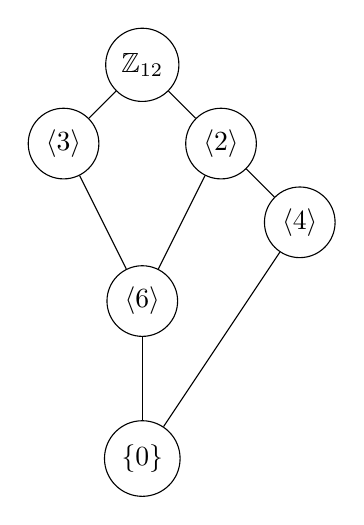
\begin{tikzpicture}
			\node[shape=circle,draw=black] (1) at (0,4) {$\Z_{12}$};
			\node[shape=circle,draw=black] (2) at (1,3) {$\langle 2\rangle$};
			\node[shape=circle,draw=black] (3) at (-1,3) {$\langle 3\rangle$};
			\node[shape=circle,draw=black] (4) at (2,2) {$\langle 4\rangle$};
			\node[shape=circle,draw=black] (6) at (0,1) {$\langle 6\rangle$};
			\node[shape=circle,draw=black] (12) at (0,-1) {$\{0\}$};
			
			\draw (1) -- (2);
			\draw (1) -- (3);
			\draw (2) -- (4);
			\draw (2) -- (6);
			\draw (3) -- (6);
			\draw (4) -- (12);
			\draw (6) -- (12);
		\end{tikzpicture}
	\end{myex}
	
	\section{Permutation groups}
	\begin{mydef}{Permutation group}{}
		Let $B=\{1, \dots, n\}$. A \underline{permutation} of $B$ is a bijection from $B$ to itself. That is to say, a function $\sigma:B\to B$ which is one-to-one and onto.
		
		Let $n\in\N$. Then, the \underline{permutation group of order $n$} is the set of all permutations on $\{1, \dots, n\}$ with the operation being function composition.
		
		Elements $\sigma$ of $S_n$ can be denoted $\sigma=\begin{pmatrix}1&2&\dots&n\\\sigma(1)&\sigma(2)&\dots&\sigma(n)\end{pmatrix}$.
	\end{mydef}
	
	\begin{myrem}{Order of $S_n$}{}
		\begin{itemize}
			\item What is $|S_n|$? Let $\sigma\in S_n$. There are $n$ possibilities for $\sigma(1)$. Given $\sigma(1)$, there are $n-1$ possibilities for $\sigma(2)$, and so on. Thus, $|S_n|=n(n-1)(n-2)\dots1=n!$.
			
			\item $S_n$ is a non-abelian group. (Prove this!)
		\end{itemize}
	\end{myrem}
	
	\subsection{Cycle notation}
	\begin{myex}{Cycle notation for elements of $S_3$}{}
		Let $\sigma=\begin{pmatrix}1&2&3\\2&1&3\end{pmatrix}$. Then, $\sigma=(12)(3)$ since $\sigma(1)=2$ and $\sigma(2)=1$ and $\sigma(3)=3$.
		
		Let $\beta=\begin{pmatrix}1&2&3\\3&1&2\end{pmatrix}$. Then, $\beta=(132)=(321)=(213)$.
	\end{myex}
	
	\begin{myex}{Cycle notation for an element of $S_6$}{}
		Let $\sigma=\begin{pmatrix}1&2&3&4&5&6\\3&4&6&2&5&1\end{pmatrix}$. Then, $\sigma=(136)(24)=(24)(136)$.
	\end{myex}
	
	\begin{mydef}{Cycles and transpositions}{}
		An expression of the form $(a_1\dots a_m)$ is a \underline{cycle length m}, and if $m=2$, a \underline{transposition}.
	\end{mydef}
	
	\begin{mythm}{Permutations are products of disjoint cycles}{}
		Let $\sigma\in S_n$. Then, $\sigma$ can be written as a cycle or a product of disjoint cycles.
		\begin{proof}
			If $\sigma$ is a cycle we're done, so suppose it's not. Then, let $a_1\in\{1, \dots, n\}$ and $a_2=\sigma(a_1), \dots, a_k=\sigma(a_{k-1}), a_1=\sigma(a_k)$. This is always possible since $\{1, \dots, n\}$ is a finite set. Let $b_1\in\{1, \dots, n\}\setminus\{a_1, \dots, a_k\}$ and $b_2=\sigma(b_1), \dots, b_m=\sigma(b_{m-1}), b_1=\sigma(b_m)$. We claim the cycles $(a_1\dots a_k)$ and $(b_1\dots b_m)$ are disjoint.
			
			For contradiction suppose $a_i=b_j$ for some $i, j$. Then,
			\begin{align*}
				\sigma^{i-1}(a_1)&=\sigma^{j-1}(b_j)\\
				b_1&=\sigma^{j-1-i+1}(a_1)\in\{a_1, \dots, a_k\}
			\end{align*}
			which is impossible since $b_1\notin\{a_1, \dots, a_k\}$.
			
			Since $\{1, \dots, n\}$ is finite, this process stops eventually, and gives a representation of $\sigma$ as a product of disjoint cycles.
		\end{proof}
	\end{mythm}
	
	\begin{myex}{}{}
		Let $\tau=(124)$, $\sigma=(1235)$. What are $\tau\sigma$ and $\sigma\tau$?
		\begin{align*}
			\tau\sigma&=(124)(1235)=(14)(235)\\
			\sigma\tau&=(135)(24)
		\end{align*}
	\end{myex}
	
	\begin{myrem}{}{}
		$S_n\leq S_m$ for $m\geq n$.
	\end{myrem}
	
	\begin{mythm}{Disjoint cycles commute}{}
		Let $\sigma=(a_1\dots a_k)$, $\tau=(b_1\dots b_l)$ be disjoint cycles. Then $\sigma\tau=\tau\sigma$.
		\begin{proof}
			We know $\{1, \dots, n\}=\{a_1, \dots, a_k\}\cup\{b_1, \dots, b_l\}\cup\{c_1, \dots, c_m\}$
			
			where $\{c_1, \dots, c_m\}=\{1, \dots, n\}\setminus(\{a_1, \dots, a_k\}\cup\{b_1, \dots, b_l\})$. So,
			\begin{itemize}
				\item For all $i\in\{1, \dots, k\}$, we have $\tau(\sigma(a_i))=\tau(a_{i+1})=a_{i+1}=\sigma(a_i)=\sigma(\tau(a_i))$ since $\tau(a_i)=a_i$.
				\item For all $i\in\{1, \dots, l\}$, we have $\sigma(\tau(b_i))=\sigma(b_{i+1})=b_{i+1}=\tau(b_i)=\tau(\sigma(b_i))$ since $\sigma(b_i)=b_i$.
				\item For all $i\in\{1, \dots, m\}$, we have $\sigma(\tau(c_i))=\sigma(c_i)=c_i=\tau(c_i)=\tau(\sigma(c_i))$ since $\sigma(c_i)\tau(c_i)=c_i$.
			\end{itemize}
			 Therefore in all cases, $\sigma\tau=\tau\sigma$.
		\end{proof}
	\end{mythm}
	
	\begin{myrem}{}{}
		Let $\sigma$ be a $k$-cycle. Then $|\sigma|=k$.
	\end{myrem}
	
	\begin{mythm}{Order of a permutation}{}
		Let $\alpha\in S_n$. Then $|\alpha|$ is the least common multiple of the lengths of the disjoint cycles representing $\alpha$.
		\begin{proof}
			Let $\sigma, \tau\in S_n$ be disjoint cycles, with $\sigma$ being an $m$-cycle and $\tau$ being a $k$-cycle. Let $l=\text{lcm}(k, m)$. We claim $n:=|\sigma\tau|=l$.
			
			Since $l=\text{lcm}(k, m)$, we have $k|l$ and $m|l$. So,
			\begin{align*}
				(\tau\sigma)^l&=\tau^l\sigma^l\\
				&=(\tau^k)^s(\sigma^m)^t
			\end{align*}
			for some $s, t\in\Z$. Now,
			\begin{align*}
				\tau^k&=e=\sigma^m\\
				(\tau\sigma)^l&=e
			\end{align*}
			so $n|l$.
		\end{proof}
	\end{mythm}
\end{document}